La valutazione sperimentale ha l'obiettivo di analizzare le prestazioni del modello sviluppato e verificare l'efficacia delle scelte progettuali introdotte durante l'adattamento della Tiny Recursive Model al gioco del Go.

Gli esperimenti sono stati organizzati considerando due dimensioni di scacchiera, $9 \times 9$ e $19 \times 19$, e due differenti modalità di selezione delle mosse: l'utilizzo diretto della policy generata dalla TRM e l'integrazione con una ricerca Negamax.

La valutazione si articola in due fasi principali. La prima riguarda l'analisi delle prestazioni del modello sul dataset di test, attraverso metriche quali la Cross-Entropy Loss e l'accuratezza Top-$k$. La seconda consiste nella valutazione pratica degli agenti attraverso partite giocate contro KataGo, con l'obiettivo di confrontare il comportamento delle due modalità di selezione delle mosse.

I risultati vengono infine analizzati mettendo a confronto le diverse configurazioni, considerando sia la qualità delle mosse e gli esiti delle partite, sia il costo computazionale introdotto dalla ricerca.

\subsection{Risultati sul dataset di test}

Al termine dell'addestramento, i checkpoint selezionati sono stati valutati sui rispettivi dataset di test. Questa fase consente di misurare la capacità del modello di individuare la mossa giocata nelle posizioni non utilizzate durante l'addestramento.

Le metriche considerate sono:

\begin{itemize}
    \item \textbf{Cross-Entropy Loss}: misura la differenza tra la distribuzione di probabilità prodotta dal modello e la mossa corretta presente nel dataset. Valori inferiori indicano una migliore corrispondenza tra le previsioni e le etichette di riferimento.
    \item \textbf{Top-1 Accuracy}: percentuale di posizioni nelle quali la mossa corretta coincide con quella avente la probabilità più elevata.
    \item \textbf{Top-3 Accuracy}: percentuale di posizioni nelle quali la mossa corretta compare tra le prime tre mosse previste.
    \item \textbf{Top-5 Accuracy}: percentuale di posizioni nelle quali la mossa corretta compare tra le prime cinque mosse previste.
\end{itemize}

\subsubsection{Risultati sul dataset 9x9}

Il modello addestrato sulla scacchiera $9 \times 9$ è stato valutato su un insieme di test composto da 41.380 posizioni. Il checkpoint utilizzato corrisponde all'epoca 50.

I risultati ottenuti sono riportati nella Tabella~\ref{tab:test_9x9}.

\begin{table}[htbp]
    \centering
    \caption{Metriche del modello sul dataset di test 9x9.}
    \label{tab:test_9x9}
    \begin{tabular}{lr}
        \hline
        \textbf{Metrica}   & \textbf{Risultato} \\
        \hline
        Posizioni di test  & 41.380             \\
        Cross-Entropy Loss & 1,7505             \\
        Top-1 Accuracy     & 46,67\%            \\
        Top-3 Accuracy     & 72,49\%            \\
        Top-5 Accuracy     & 83,48\%            \\
        \hline
    \end{tabular}
\end{table}

La Top-1 Accuracy indica che il modello individua direttamente la mossa corretta in circa il 46,67\% delle posizioni. Considerando invece le prime cinque previsioni, la percentuale sale all'83,48\%.

\subsubsection{Risultati sul dataset 19x19}

Per la scacchiera $19 \times 19$, la valutazione è stata effettuata su un insieme di test composto da 208.653 posizioni. Il checkpoint utilizzato corrisponde all'epoca 10.

I risultati sono riportati nella Tabella~\ref{tab:test_19x19}.

\begin{table}[htbp]
    \centering
    \caption{Metriche del modello sul dataset di test 19x19.}
    \label{tab:test_19x19}
    \begin{tabular}{lr}
        \hline
        \textbf{Metrica}   & \textbf{Risultato} \\
        \hline
        Posizioni di test  & 208.653            \\
        Cross-Entropy Loss & 2,6234             \\
        Top-1 Accuracy     & 36,20\%            \\
        Top-3 Accuracy     & 56,72\%            \\
        Top-5 Accuracy     & 65,47\%            \\
        \hline
    \end{tabular}
\end{table}

Anche in questo caso l'accuratezza aumenta considerando un insieme più ampio di mosse candidate. La Top-5 Accuracy raggiunge il 65,47\%, mentre la Top-1 si attesta al 36,20\%.

\subsubsection{Confronto tra le due configurazioni}

La Figura~\ref{fig:test_topk_accuracy} mette a confronto le accuratezze Top-$k$ ottenute sulle due dimensioni della scacchiera.

\begin{figure}[htbp]
    \centering
    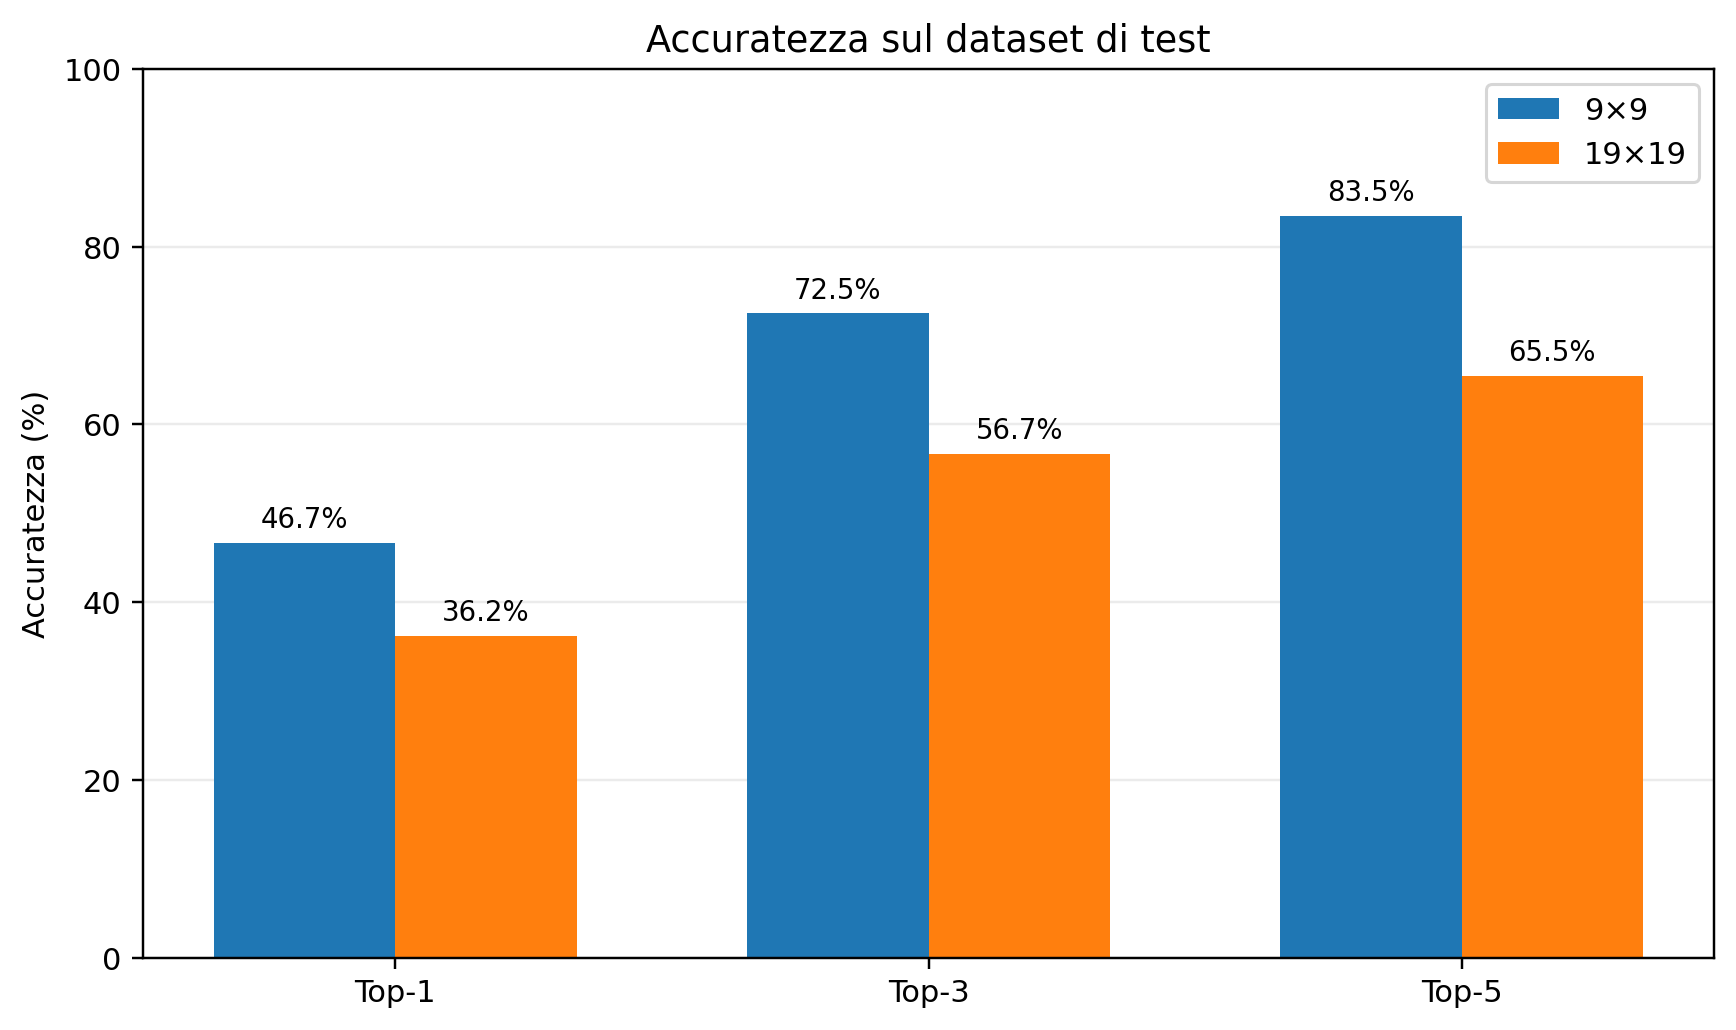
\includegraphics[width=0.85\textwidth]{img/test_accuracy_topk.png}
    \caption{Confronto tra le accuratezze Top-1, Top-3 e Top-5 sui dataset di test.}
    \label{fig:test_topk_accuracy}
\end{figure}

I risultati mostrano prestazioni superiori per la configurazione $9 \times 9$ rispetto a quella $19 \times 19$ su tutte le metriche considerate. Questa differenza deve tuttavia essere interpretata tenendo conto delle diverse dimensioni degli spazi di azione: il modello 9x9 deve scegliere tra 82 azioni, mentre quello 19x19 tra 362.

Inoltre, i due modelli sono stati addestrati su dataset distinti, con un diverso numero di esempi e caratteristiche proprie. Le differenze osservate non possono quindi essere attribuite esclusivamente alla dimensione della scacchiera.

Un ulteriore elemento riguarda la previsione della mossa PASS. Nel dataset di test 9x9 sono presenti 607 esempi PASS, mentre nel dataset 19x19 ne sono presenti 683. Le metriche specifiche di questa classe mostrano risultati differenti: sul 9x9 la precisione è pari al 67,45\% e il recall al 76,11\%; sul 19x19 la precisione raggiunge l'80,68\%, mentre il recall è pari al 55,64\%.

Questi valori evidenziano che la capacità di riconoscere correttamente una mossa di PASS non coincide necessariamente con la capacità di individuare le altre mosse. La distinzione è rilevante, poiché la scelta anticipata di PASS può influenzare significativamente lo svolgimento di una partita.

\subsection{Valutazione contro KataGo}

Per valutare il comportamento degli agenti durante una partita completa, sono stati eseguiti esperimenti contro KataGo, utilizzato come avversario di riferimento.

Per ciascuna dimensione della scacchiera sono state confrontate due configurazioni:
\begin{itemize}
    \item \textbf{Policy}: l'agente seleziona le mosse direttamente dalla distribuzione di probabilità prodotta dalla TRM, dopo aver escluso le azioni illegali.
    \item \textbf{Negamax}: la policy della TRM viene utilizzata per ordinare le mosse candidate, sulle quali viene applicata una ricerca Negamax con potatura alpha-beta.
\end{itemize}

L'obiettivo è verificare se l'introduzione di una ricerca limitata possa migliorare le prestazioni dell'agente rispetto all'utilizzo diretto della policy.

\subsubsection{Configurazione degli esperimenti}

Per ciascuna delle quattro configurazioni sono state giocate 100 partite contro KataGo, alternando il colore assegnato al TRM: 50 partite con il Nero e 50 con il Bianco.

Gli esperimenti sono stati eseguiti utilizzando i seguenti parametri:

\begin{table}[htbp]
    \centering
    \caption{Parametri comuni agli esperimenti contro KataGo.}
    \label{tab:katago_common_config}
    \begin{tabular}{ll}
        \hline
        \textbf{Parametro}         & \textbf{Valore}    \\
        \hline
        Partite per configurazione & 100                \\
        Visite massime KataGo      & 40                 \\
        Profilo HumanSL            & rank\_20k          \\
        Seed                       & 42                 \\
        Komi                       & 7,5                \\
        Penalità sul logit PASS    & 3,5                \\
        Soglia penalità PASS       & 16 pietre occupate \\
        Ricerca Negamax            & Profondità 2       \\
        Candidati Negamax 9x9      & 5                  \\
        Candidati Negamax 19x19    & 3                  \\
        \hline
    \end{tabular}
\end{table}

Per entrambe le dimensioni è stato utilizzato il profilo HumanSL di KataGo denominato \texttt{rank\_20k}. È quindi opportuno precisare che il confronto non è stato effettuato con KataGo alla sua massima forza, ma con una configurazione basata sul profilo umano indicato.

I modelli KataGo utilizzati sono differenti in funzione della dimensione della scacchiera: per il 9x9 è stato impiegato il modello \texttt{kata9x9-b18c384nbt-20231025}, mentre per il 19x19 è stato utilizzato \texttt{kata1-tf3-b11c768-s12382M-d6533M}.

Le partite sono state giocate applicando le regole di scoring ad area, il positional superko e il divieto di suicidio. Il komi è stato impostato a 7,5 punti.

Per confrontare gli agenti sono state considerate principalmente le seguenti metriche:
\begin{itemize}
    \item numero di vittorie, pareggi e sconfitte;
    \item percentuale di vittorie del TRM;
    \item margine medio e mediano delle partite, calcolato dal punto di vista del TRM;
    \item numero medio di mosse per partita;
    \item durata complessiva degli esperimenti e, per Negamax, statistiche della ricerca.
\end{itemize}

Il margine, indicato nel seguito come \textit{gap}, è calcolato sottraendo il punteggio finale di KataGo da quello del TRM. Un valore positivo indica quindi una vittoria o un vantaggio del TRM, mentre un valore negativo indica un vantaggio di KataGo.

\subsubsection{Risultati sul 9x9}

I risultati delle partite sulla scacchiera $9 \times 9$ sono riportati nella Tabella~\ref{tab:katago_9x9}.

\begin{table}[htbp]
    \centering
    \caption{Risultati degli esperimenti contro KataGo sul 9x9.}
    \label{tab:katago_9x9}
    \begin{tabular}{lrr}
        \hline
        \textbf{Metrica} & \textbf{Policy} & \textbf{Negamax} \\
        \hline
        Vittorie TRM     & 26              & 58               \\
        Pareggi          & 0               & 0                \\
        Sconfitte TRM    & 74              & 42               \\
        Win rate         & 26,0\%          & 58,0\%           \\
        Gap medio        & -13,4           & -24,8            \\
        Gap mediano      & -11,5           & +1,5             \\
        Mosse medie      & 64,0            & 98,7             \\
        Durata test      & 2,7 min         & 4,3 min          \\
        \hline
    \end{tabular}
\end{table}

L'introduzione della ricerca Negamax produce un incremento significativo della percentuale di vittorie, che passa dal 26\% al 58\%. La configurazione con ricerca ottiene quindi 32 punti percentuali in più rispetto all'utilizzo diretto della policy.

Si osserva inoltre un aumento del numero medio di mosse per partita, che passa da 64,0 a 98,7. Questo risultato indica che le partite giocate dall'agente con Negamax tendono a proseguire più a lungo.

Il margine medio rimane tuttavia negativo in entrambe le configurazioni. Nel caso di Negamax, la differenza tra margine medio e mediano è particolarmente evidente: il valore mediano è positivo, mentre quello medio è negativo. Ciò suggerisce la presenza di alcune sconfitte con margini particolarmente ampi, capaci di influenzare il valore medio nonostante il maggior numero di vittorie.

\subsubsection{Risultati sul 19x19}

La Tabella~\ref{tab:katago_19x19} riporta i risultati ottenuti sulla scacchiera $19 \times 19$.

\begin{table}[htbp]
    \centering
    \caption{Risultati degli esperimenti contro KataGo sul 19x19.}
    \label{tab:katago_19x19}
    \begin{tabular}{lrr}
        \hline
        \textbf{Metrica} & \textbf{Policy} & \textbf{Negamax} \\
        \hline
        Vittorie TRM     & 48              & 65               \\
        Pareggi          & 0               & 0                \\
        Sconfitte TRM    & 52              & 35               \\
        Win rate         & 48,0\%          & 65,0\%           \\
        Gap medio        & -1,3            & -62,8            \\
        Gap mediano      & -0,5            & +3,5             \\
        Mosse medie      & 216,5           & 393,8            \\
        Durata test      & 17,6 min        & 35,7 min         \\
        \hline
    \end{tabular}
\end{table}

Anche sulla scacchiera $19 \times 19$ la ricerca Negamax determina un incremento della percentuale di vittorie, che passa dal 48\% al 65\%, con un miglioramento di 17 punti percentuali.

Il numero medio di mosse per partita aumenta da 216,5 a 393,8. L'introduzione della ricerca comporta quindi partite mediamente più lunghe e un maggiore costo computazionale.

Anche in questa configurazione si osserva una differenza tra margine medio e mediano. In particolare, il margine medio di Negamax è pari a -62,8 punti, mentre quello mediano è pari a +3,5 punti. Il valore medio risulta pertanto influenzato da alcune sconfitte particolarmente ampie, nonostante il numero complessivo di vittorie sia superiore a quello della policy diretta.

\subsubsection{Confronto tra Policy e Negamax}

La Figura~\ref{fig:katago_winrate} riassume le percentuali di vittoria ottenute nelle quattro configurazioni sperimentali.

\begin{figure}[htbp]
    \centering
    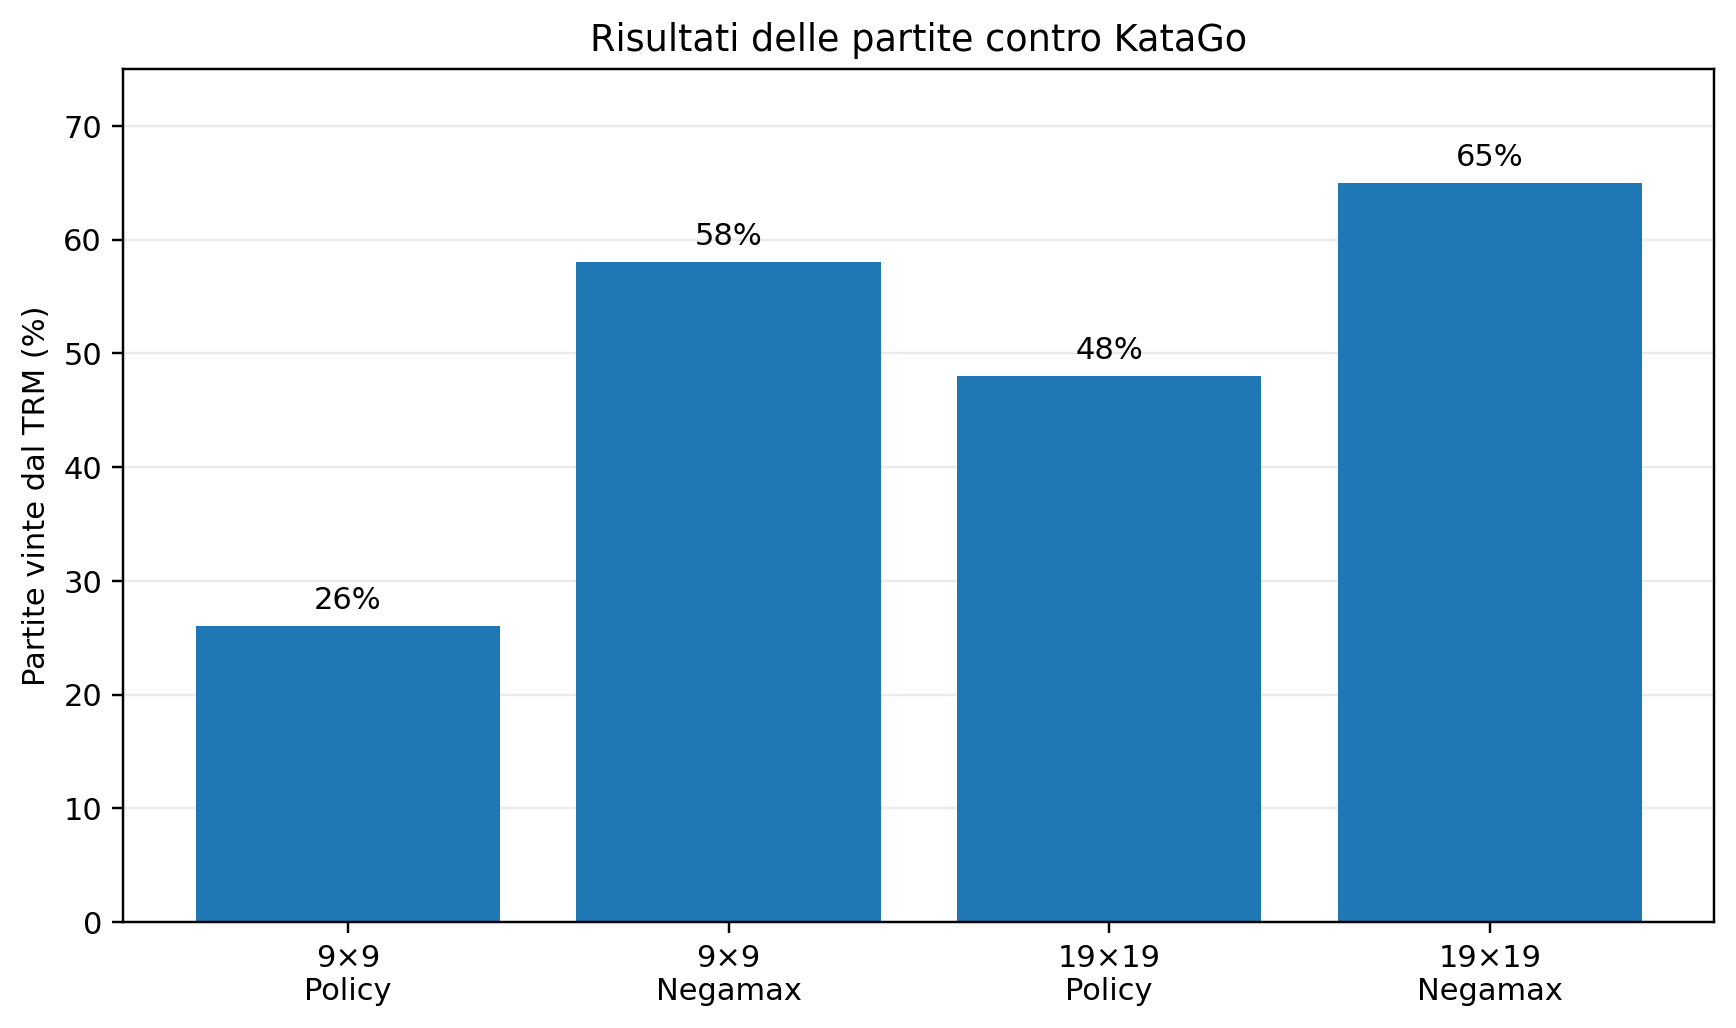
\includegraphics[width=0.85\textwidth]{img/win_rate_katago.png}
    \caption{Percentuale di vittorie del TRM contro KataGo nelle quattro configurazioni sperimentali.}
    \label{fig:katago_winrate}
\end{figure}

In entrambe le dimensioni della scacchiera, l'integrazione della ricerca Negamax migliora la percentuale di vittorie rispetto all'utilizzo diretto della policy.

Il miglioramento è particolarmente evidente nel caso del 9x9, dove la percentuale di vittorie passa dal 26\% al 58\%. Nel caso del 19x19 si osserva invece un incremento dal 48\% al 65\%.

È tuttavia importante considerare che l'aumento delle vittorie non si traduce necessariamente in un miglioramento del margine medio. Come mostrano le tabelle precedenti, alcune sconfitte hanno margini particolarmente elevati e influenzano negativamente la media.

Un ulteriore aspetto riguarda il costo della ricerca. Nel caso del 9x9, il tempo complessivo dedicato alla ricerca Negamax è stato pari a 79,89 secondi, con 123.573 nodi esplorati e 92.770 foglie valutate. Per il 19x19, il tempo complessivo di ricerca è stato pari a 899,38 secondi, con 301.538 nodi esplorati e 218.254 foglie valutate.

Questi valori evidenziano come l'aumento della dimensione della scacchiera comporti un costo computazionale maggiore, anche a parità di profondità di ricerca. La ricerca Negamax permette quindi di migliorare le prestazioni in termini di vittorie, introducendo però un maggiore costo in termini di tempo di esecuzione.

\subsection{Analisi dei risultati e considerazioni}

I risultati ottenuti permettono di formulare alcune considerazioni sull'adattamento della Tiny Recursive Model al gioco del Go.

In primo luogo, la valutazione sui dataset di test mostra che il modello è in grado di individuare la mossa corretta con una certa frequenza, soprattutto considerando un insieme di mosse candidate anziché la sola previsione principale. Le prestazioni risultano differenti tra le due dimensioni della scacchiera, evidenziando la maggiore difficoltà associata allo spazio di azione più ampio del 19x19.

La valutazione contro KataGo evidenzia inoltre un miglioramento della percentuale di vittorie quando la policy viene integrata con una ricerca Negamax. Tale risultato suggerisce che l'utilizzo delle probabilità prodotte dalla TRM per guidare una ricerca limitata può contribuire a migliorare la selezione delle mosse rispetto all'utilizzo diretto della policy.

D'altra parte, i margini medi delle partite mostrano che il numero di vittorie non è sufficiente, da solo, a descrivere completamente le prestazioni dell'agente. In particolare, le differenze tra media e mediana evidenziano la presenza di partite perse con margini molto ampi, che incidono significativamente sul risultato complessivo.

Infine, la ricerca Negamax comporta un aumento del tempo di esecuzione e del numero di operazioni necessarie per selezionare una mossa. Questo aspetto evidenzia il compromesso tra qualità delle decisioni e costo computazionale: una ricerca più articolata può migliorare il comportamento dell'agente, ma richiede risorse aggiuntive.

Nel complesso, gli esperimenti mostrano che la TRM può essere adattata al gioco del Go e utilizzata come componente di una policy per la selezione delle mosse. L'integrazione con una ricerca Negamax limitata rappresenta un ulteriore miglioramento pratico, pur lasciando emergere limiti nella qualità delle decisioni e nella gestione delle situazioni strategicamente più complesse.
